Este problema conciste en generar la silueta de una ciudad a partir de la representacion de varios edificios que la componen.
A la entrada del algoritmo voy a tener una cantidad textbf{N} de edificios, representados con tres valores; en donde comienza, su altura y dode termina. Todos los valores son enteros positivos, en relacion los texttt{ceros} de cada eje, horizontal y longitudinal.
A la salida voy a tener representada la silueta de la ciudad como una seguidillas de puntos que representan el contorno de los edificios que textbf{sobresalen} del resto.
La gracia de todo esto es ocultar las partes de los edificios que quedan textbf{dentro} de otros edificios.

\subsubsection*{Escenarios t\'ipicos}
\addcontentsline{toc}{subsubsection}{Escenarios t\'ipicos}

Las siguientes instancias son las b\'asicas a las cuales se pueden reducir todos los escenarios.

\subsubsection*{Edificio B\'asico}
\addcontentsline{toc}{subsubsection}{Edificio B\'asico}
\begin{figure}[H]
\begin{center}$
\begin{array}{cc}
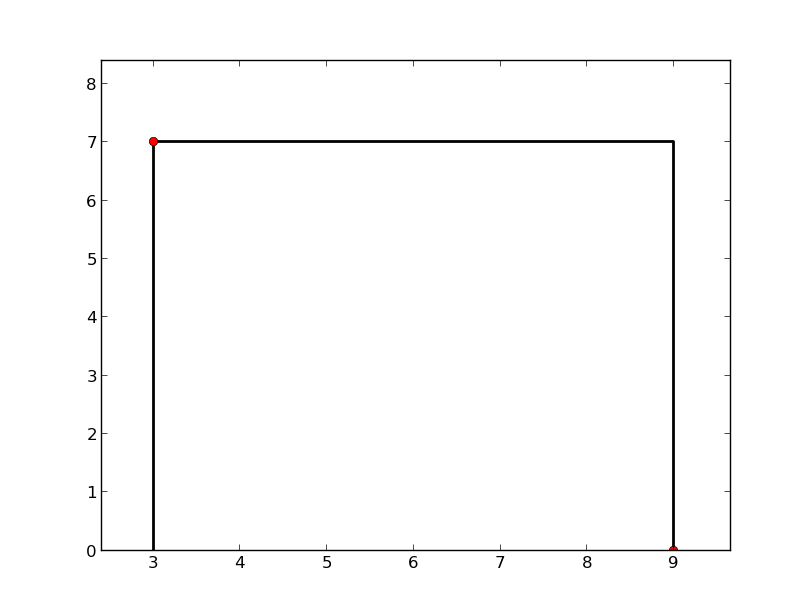
\includegraphics[scale=0.35]{./imagenes/ej2_edificio1.png}&
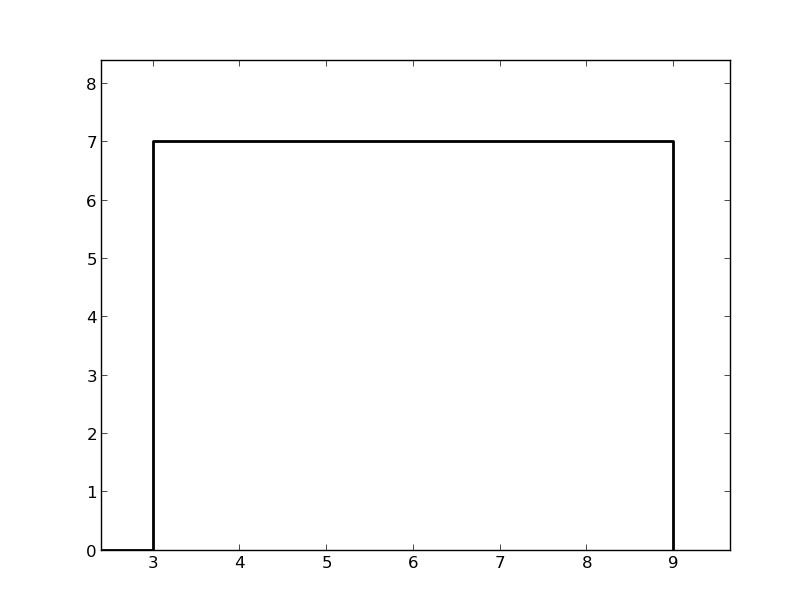
\includegraphics[scale=0.35]{./imagenes/ej2_edificio1solucion.png}
\end{array}$
\end{center}
\caption{Una ciudad con un solo edificio}
\end{figure}

\subsubsection*{Edificios Cruzados 1}
\addcontentsline{toc}{subsubsection}{Edificios Cruzados 1}
\begin{figure}[H]
\begin{center}$
\begin{array}{cc}
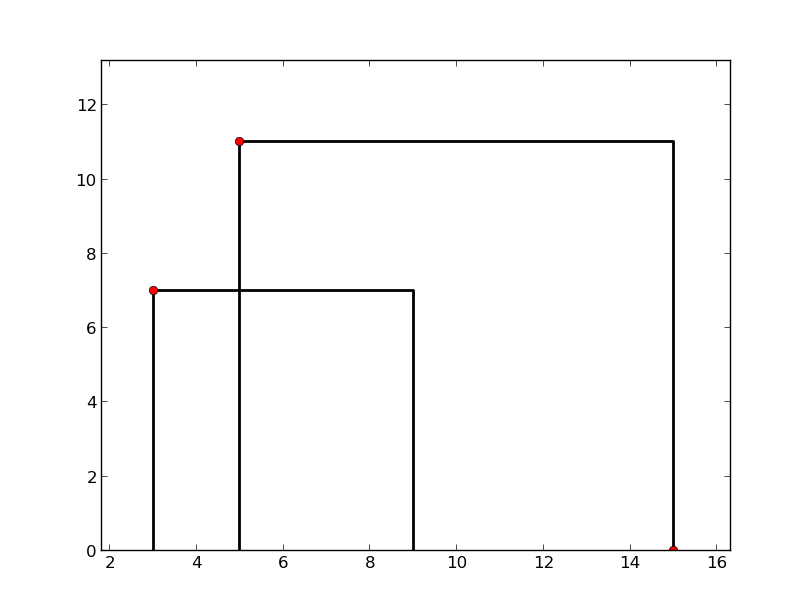
\includegraphics[scale=0.35]{./imagenes/ej2_edificio2.png}&
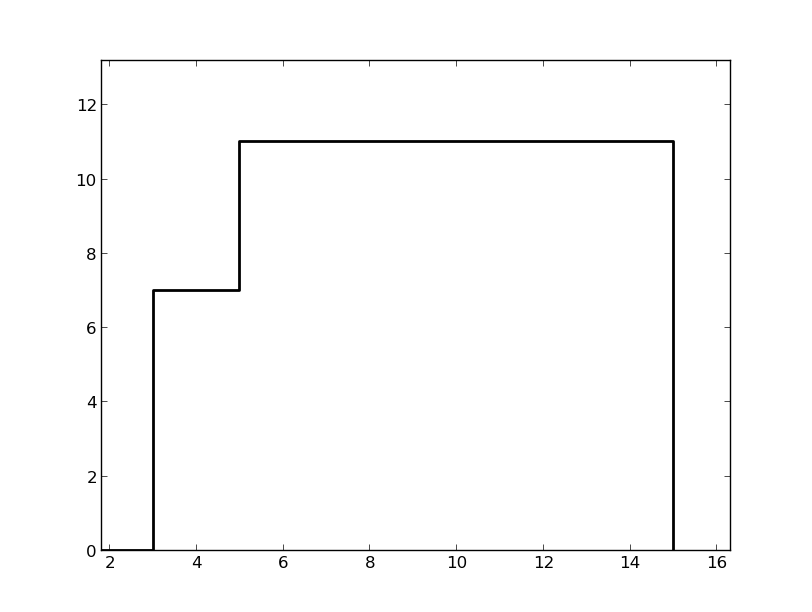
\includegraphics[scale=0.35]{./imagenes/ej2_edificio2solucion.png}
\end{array}$
\end{center}
\caption{Edificios Cruzados 1}
\end{figure}

\subsubsection*{Edificios Cruzados 2}
\addcontentsline{toc}{subsubsection}{Edificios Cruzados 2}
\begin{figure}[H]
\begin{center}$
\begin{array}{cc}
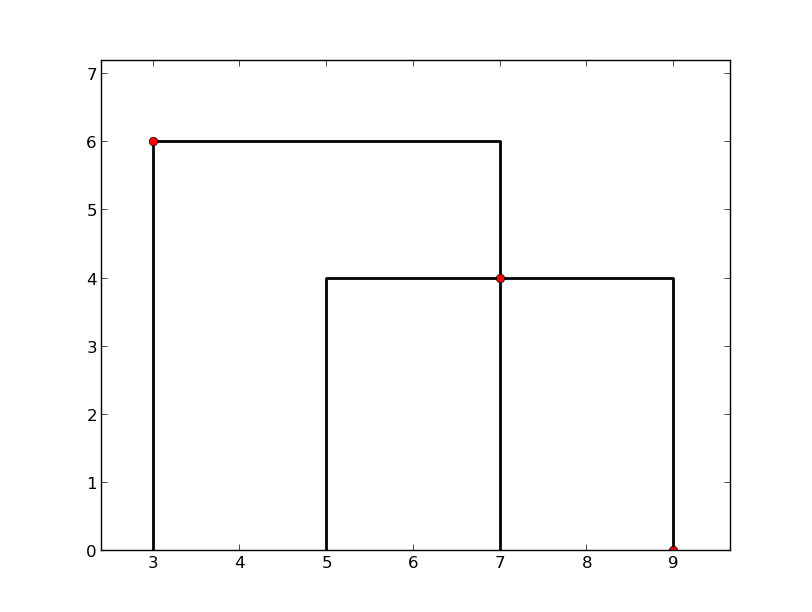
\includegraphics[scale=0.35]{./imagenes/ej2_edificio3.png}&
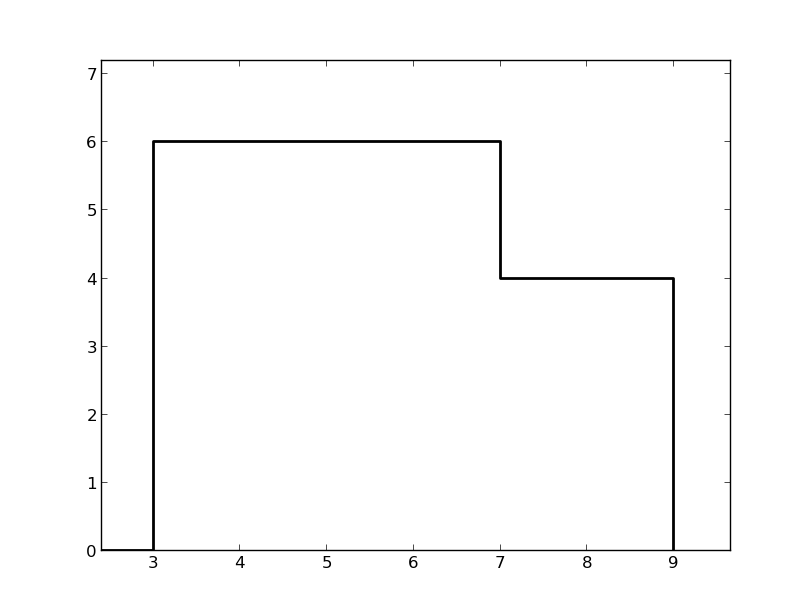
\includegraphics[scale=0.35]{./imagenes/ej2_edificio3solucion.png}
\end{array}$
\end{center}
\caption{Edificios Cruzados 2}
\end{figure}

\subsubsection*{Edificios Solapados}
\addcontentsline{toc}{subsubsection}{Edificios Solapados}
\begin{figure}[H]
\begin{center}$
\begin{array}{cc}
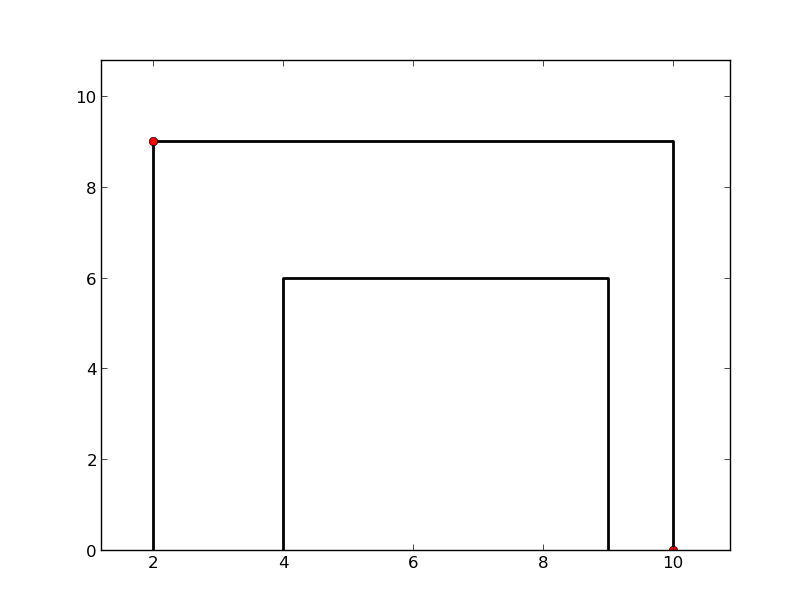
\includegraphics[scale=0.35]{./imagenes/ej2_edificio4.png}&
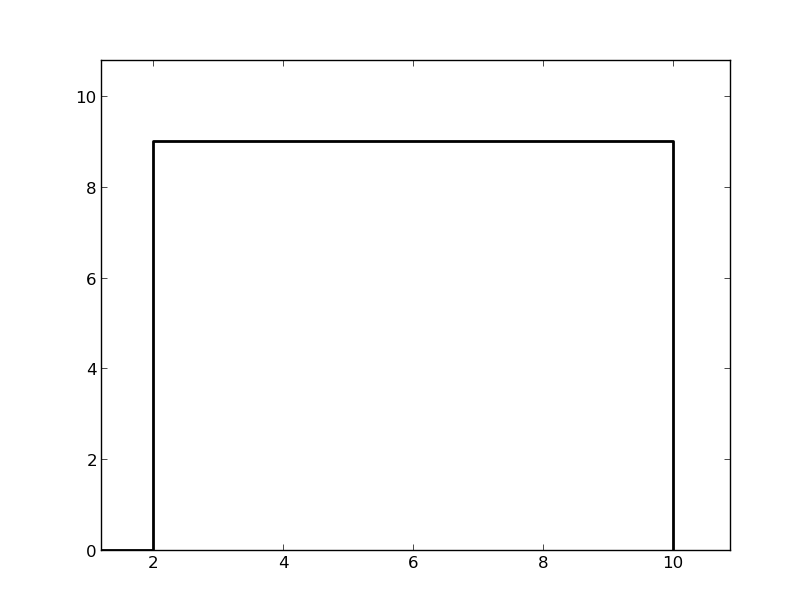
\includegraphics[scale=0.35]{./imagenes/ej2_edificio4solucion.png}
\end{array}$
\end{center}
\caption{Edificios Solapados}
\end{figure}

\subsubsection*{Edificios Contiguos}
\addcontentsline{toc}{subsubsection}{Edificios Contiguos}
\begin{figure}[H]
\begin{center}$
\begin{array}{cc}
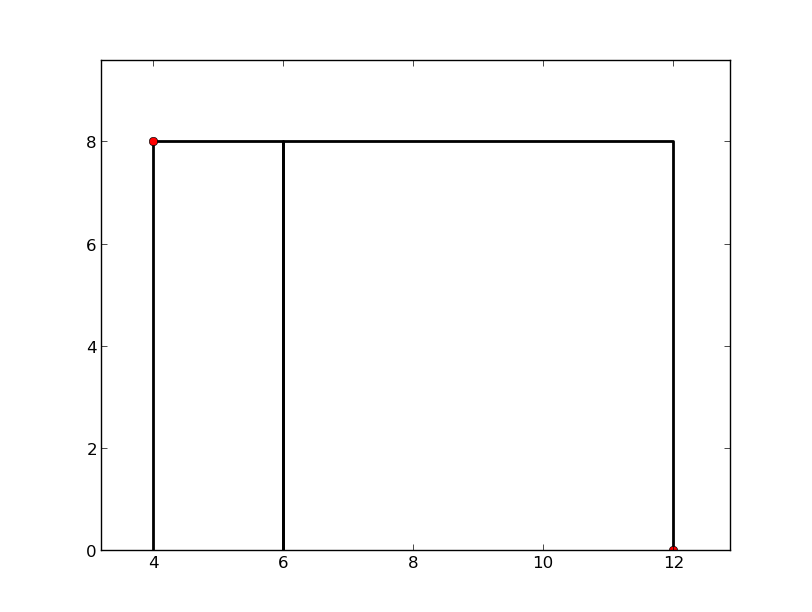
\includegraphics[scale=0.35]{./imagenes/ej2_edificio5.png}&
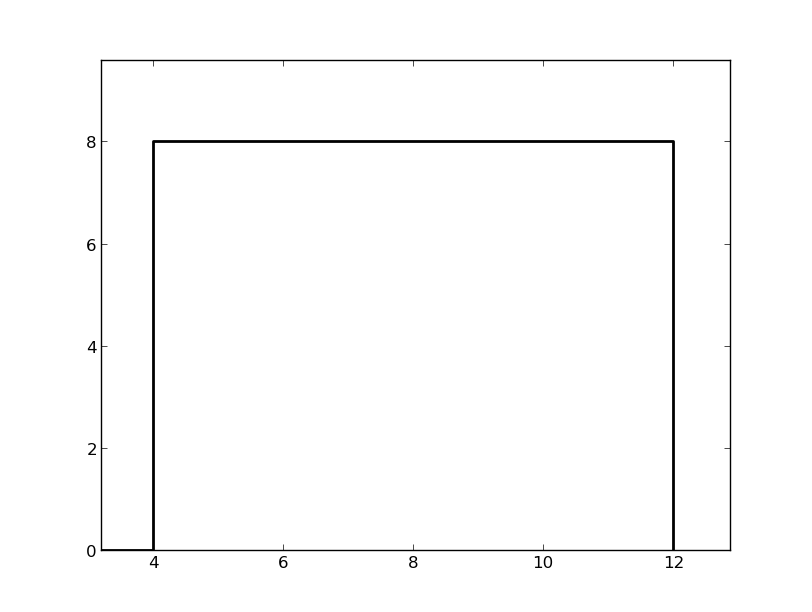
\includegraphics[scale=0.35]{./imagenes/ej2_edificio5solucion.png}
\end{array}$
\end{center}
\caption{Edificios Contiguos}
\end{figure}


\subsubsection*{Edificios Varios}
\addcontentsline{toc}{subsubsection}{Edificios Varios}
\begin{figure}[H]
\begin{center}$
\begin{array}{cc}
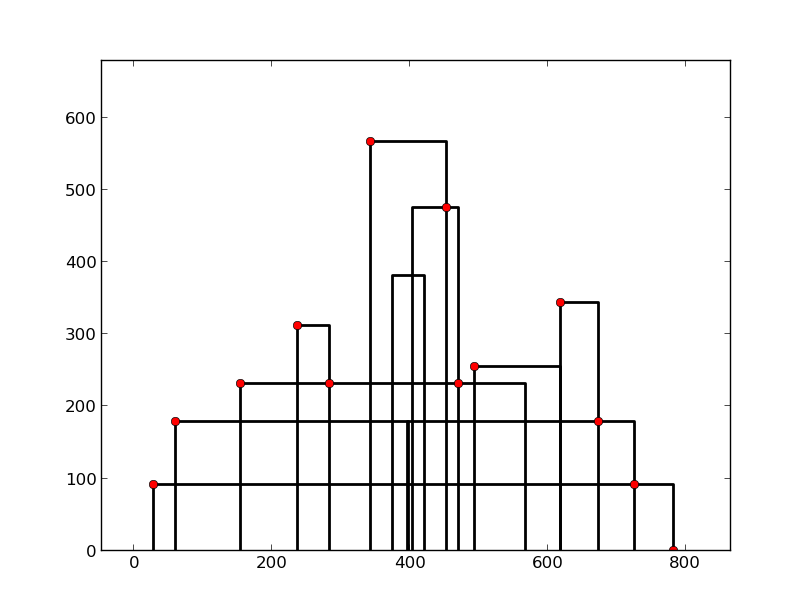
\includegraphics[scale=0.35]{./imagenes/ej2_edificio6.png}&
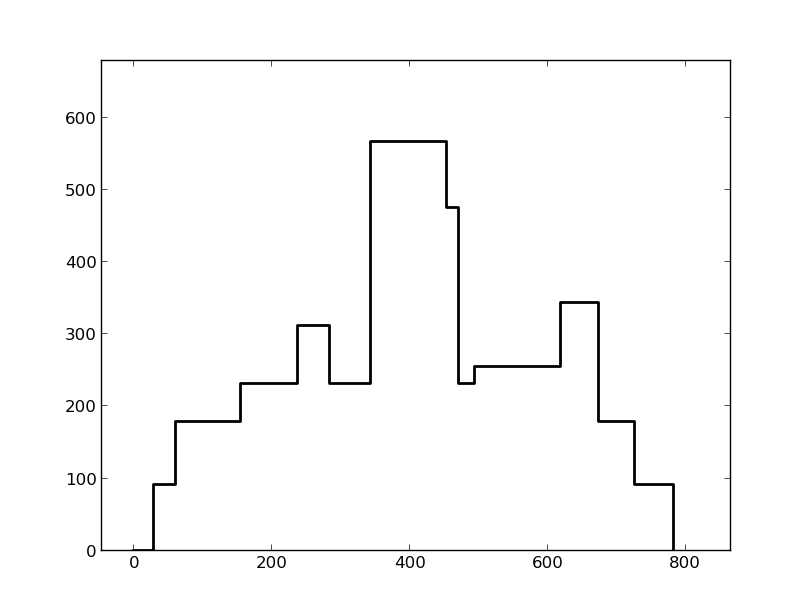
\includegraphics[scale=0.35]{./imagenes/ej2_edificio6solucion.png}
\end{array}$
\end{center}
\caption{Edificios Varios}
\end{figure}